\documentclass{article}
\usepackage[utf8]{inputenc}
\usepackage[table,xcdraw]{xcolor}

% for Polish language
\usepackage[T1]{fontenc}

% for figures
\usepackage{graphicx}

% For the Gantt chart
\usepackage{multirow}
\usepackage{pdflscape}
\usepackage{colortbl}
\usepackage{tabulary}
\usepackage{etoolbox}
\newcommand{\bcell}{\cellcolor[HTML]{000000}}
\newcommand{\gcell}{\cellcolor[HTML]{808080}}

% For the bibliography
\renewcommand{\refname}{Project literature}

% For the latex numbering
\usepackage{enumitem}
\setlist{nolistsep}

% For URLs
\usepackage{hyperref}

% For footnotes in tables
\usepackage{tablefootnote}

% For the margins
\usepackage[a4paper, total={6in, 9in}]{geometry}

\title{Individual Research Plan}
\author{John Brown}
\date{August 2022}

\begin{document}

\maketitle
% \tableofcontents

\section{Basic Data}

% Basic information on the doctoral student and the doctoral dissertation underway. In the case of a supervisor from outside Wrocław University of Science and Technology, affiliation should be provided.

\begin{table}[ht]
    \centering
    \begin{tabular}{|p{1.8in}|l|}
    \hline
     \textbf{Name, surname} &  \\ \hline
     \textbf{Discipline of education} &  \\ \hline
     \textbf{Faculty} &  \\ \hline
     \textbf{Department} &  \\ \hline
     \textbf{Date of commencement of the doctoral education} &  \\ \hline
     \textbf{ORCID No.} &  \\ \hline
     \textbf{Supervisor(s)} &  \\ \hline
     \textbf{Assistant supervisor} &  \\ \hline
    \end{tabular}
\end{table}


\section{Topic of doctoral dissertation}

% Proposed topic for a doctoral dissertation. The presented topic does not have to constitute the final title of the doctoral dissertation submitted at the end of education at the Doctoral School.

Sed ut perspiciatis, unde omnis iste natus error sit voluptatem accusantium doloremque laudantium, totam rem aperiam eaque ipsa, quae ab illo inventore veritatis et quasi architecto beatae vitae dicta sunt, explicabo.


\section{Schedule for the preparation of the doctoral dissertation}

% A schedule for the preparation of the doctoral dissertation detailing the stages and locations of the research to be conducted, including the dates for completing the sub-studies and developing their results, and optionally, depending on the type of research to be conducted, selected among the following:
% * execution of the research (including preparation of the research site, preparation of materials for the research, execution of measurements/experiments, elaboration of the obtained results),
% * preparation and submission of a scientific article to the editor of a scientific journal, 
% * submission of a patent application to the relevant office, 
% * development of an implementation proposal for the industry,
% * participation in conferences, workshops or summer/winter schools and presentation of research results,
% * preparation of an application and application for a scholarship,
% * domestic or foreign mobility of the doctoral student (including scientific consultations and study visits to domestic or foreign centres).

\begin{table}[ht]
    \centering
    \begin{tabular}{|p{1.1in}|p{4.5in}|}
    \hline
    \textbf{Task implementation period} & \multicolumn{1}{c|}{\textbf{Brief description of the task}} \\ \hline \hline
    Semester 1 &  \\ \hline
    Semester 2 &  \\ \hline
    Semester 3 &  \\ \hline
    Semester 4 &  \\ \hline
    Semester 5 &  \\ \hline
    Semester 6 &  \\ \hline
    Semester 7 &  \\ \hline
    Semester 8 &  \\ \hline
    \end{tabular}
\end{table}


\section{Date of the doctoral dissertation submission}

% A planned date for submission of the dissertation, which must not exceed the date of completion of the eighth semester of education in the Doctoral School.

\begin{center}
    \large September 202X
\end{center}

\section{Justification for choosing the topic of the doctoral dissertation}

% Description containing the justification for the selection of the topic of the doctoral dissertation, taking into account the potential areas of application of the planned results of the doctoral dissertation (at most 1 page, font 11, line spacing 1).

Sed ut perspiciatis, unde omnis iste natus error sit voluptatem accusantium doloremque laudantium, totam rem aperiam eaque ipsa, quae ab illo inventore veritatis et quasi architecto beatae vitae dicta sunt, explicabo.

\section{Outline of the current state of research in the topic of the doctoral dissertation}

% A literature review containing a description of the current state of research in the subject of the doctoral dissertation, including references to the most important literature items related to the subject of the doctoral dissertation (at most 2 pages, font 11, line spacing 1).

Sed ut perspiciatis, unde omnis iste natus error sit voluptatem accusantium doloremque laudantium, totam rem aperiam eaque ipsa, quae ab illo inventore veritatis et quasi architecto beatae vitae dicta sunt, explicabo.

\begin{figure}
    \centering
    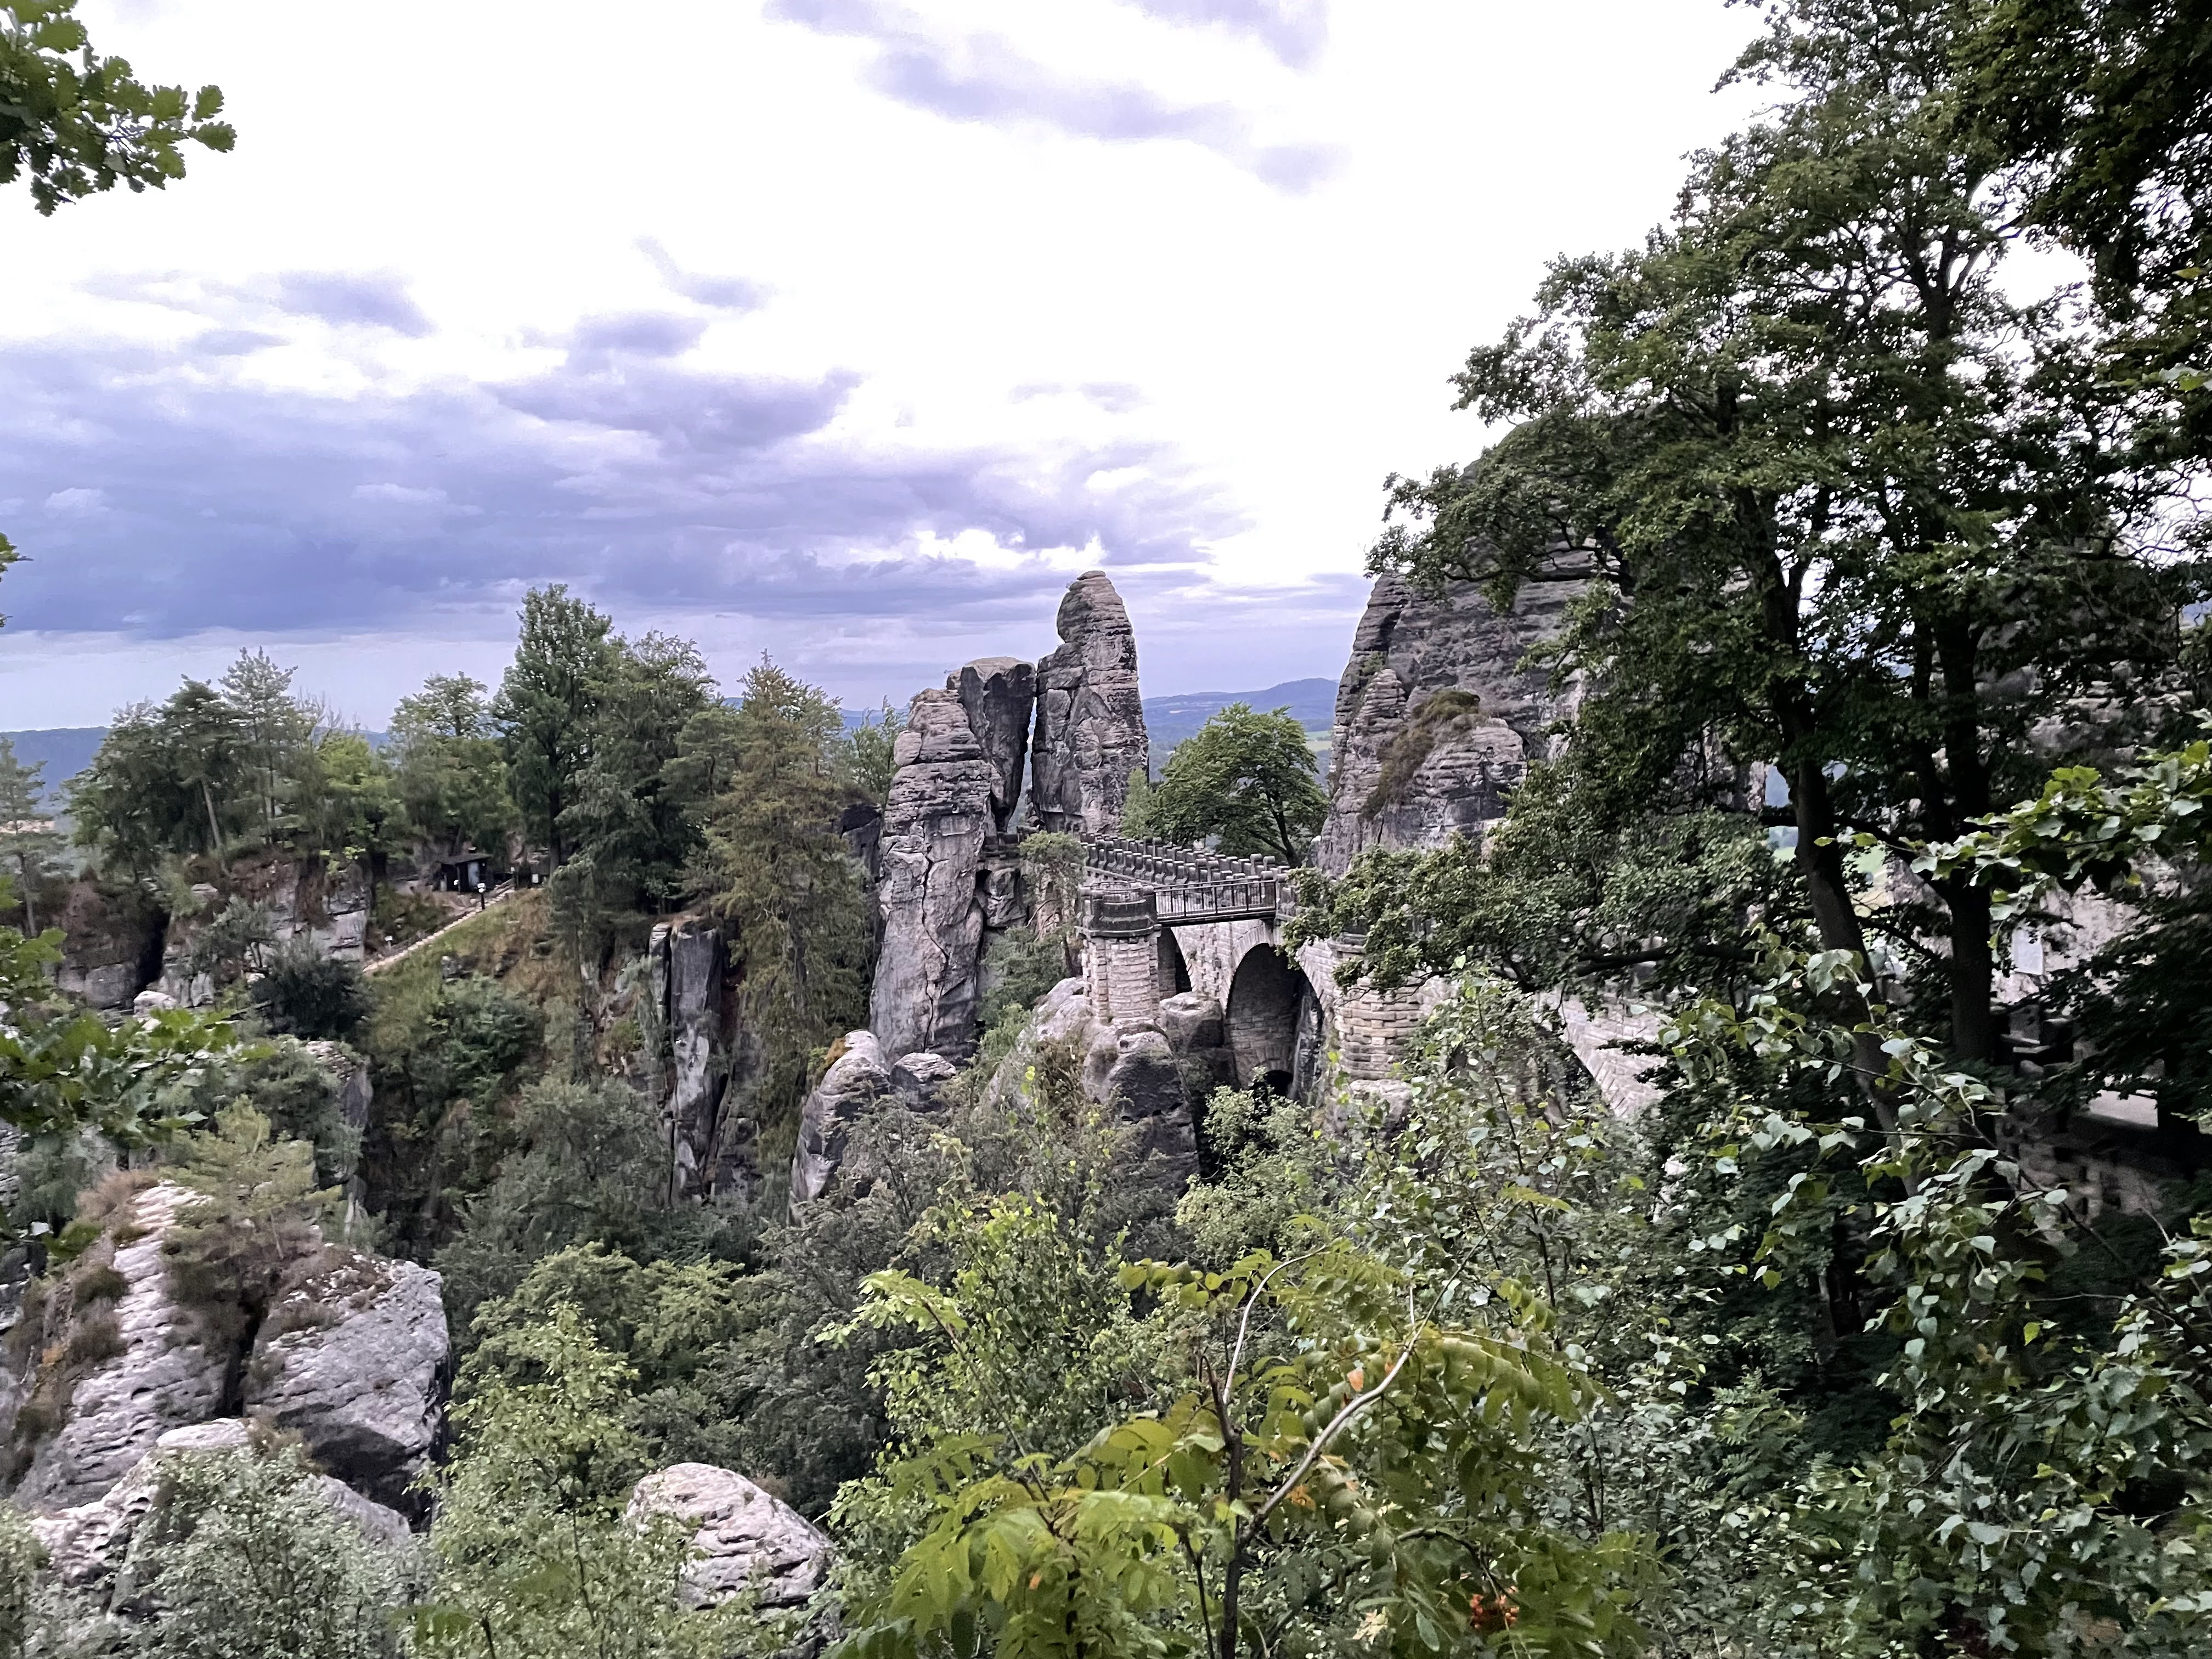
\includegraphics[width=\textwidth]{graphics/image.jpg}
    \caption{My Image}
    \label{fig:my_label}
\end{figure}
\section{Research questions and hypotheses}

% Description of the most important research questions and hypotheses related to the doctoral dissertation (at most 1 page, font 11, line spacing 1).

Sed ut perspiciatis, unde omnis iste natus error sit voluptatem accusantium doloremque laudantium, totam rem aperiam eaque ipsa, quae ab illo inventore veritatis et quasi architecto beatae vitae dicta sunt, explicabo.

\section{Contribution of the expected results to development of scientific discipline}

% Brief description of the expected contribution of the results of the doctoral dissertation to the development of the scientific discipline in which the doctoral dissertation is carried out (at most 1 page, font 11, line spacing 1).

Sed ut perspiciatis, unde omnis iste natus error sit voluptatem accusantium doloremque laudantium, totam rem aperiam eaque ipsa, quae ab illo inventore veritatis et quasi architecto beatae vitae dicta sunt, explicabo.

\section{Planned research methods}

% Brief description of the research methods that will be used during the implementation of the doctoral dissertation (at most 2 pages, font 11, line spacing 1).

Sed ut perspiciatis, unde omnis iste natus error sit voluptatem accusantium doloremque laudantium, totam rem aperiam eaque ipsa, quae ab illo inventore veritatis et quasi architecto beatae vitae dicta sunt, explicabo.

\section{Abstract for general public}

% The description for general public must be in Polish and in English. The language versions must be identical. The description should be written for general public and should include the doctoral dissertation goal, description of research, reasons for attempting a particular research topic and substantial results expected (at most 1 page, font 11, line spacing 1).

\subsection{Polish version}

Sed ut perspiciatis, unde omnis iste natus error sit voluptatem accusantium doloremque laudantium, totam rem aperiam eaque ipsa, quae ab illo inventore veritatis et quasi architecto beatae vitae dicta sunt, explicabo.

\subsection{English version}

Sed ut perspiciatis, unde omnis iste natus error sit voluptatem accusantium doloremque laudantium, totam rem aperiam eaque ipsa, quae ab illo inventore veritatis et quasi architecto beatae vitae dicta sunt, explicabo.

\section{Date of submission for publication of at least one scientific article or monography}

% A date of submission for publication of at least one scientific article published in a scientific journal or in the peer-reviewed materials of an international conference in the relevant scientific discipline, which in the year of publication of the article in its final form were included in the list drawn up in accordance with the regulations issued under the Act (Art. 267 sec. 2 point 2(b) or 1 scientific monograph published by a publishing house, which in the year of publication of the monograph in its final form was included in the list drawn up in accordance with the regulations issued pursuant to the Act (Art. 267 sec. 2 point 2(a), referred to in Art. 186 sec. 1 point 3 of the Act.

\begin{center}
    \large February 202Y
\end{center}

\section{Other comments}

% Additional explanations, comments, summary related to the individual research plan (at most 1 page, font 11, line spacing 1).

Sed ut perspiciatis, unde omnis iste natus error sit voluptatem accusantium doloremque laudantium, totam rem aperiam eaque ipsa, quae ab illo inventore veritatis et quasi architecto beatae vitae dicta sunt, explicabo.


\section{Planned form of cooperation with the supervisor}

% Brief description of the planned form of cooperation with the supervisor, e.g., frequency of meetings, form of meetings and their scope, method of communication

Sed ut perspiciatis, unde omnis iste natus error sit voluptatem accusantium doloremque laudantium, totam rem aperiam eaque ipsa, quae ab illo inventore veritatis et quasi architecto beatae vitae dicta sunt, explicabo.


\section{Opinion of assistant supervisor}

% Assistant supervisor (if appointed) should provide an opinion of the IRP.

Sed ut perspiciatis, unde omnis iste natus error sit voluptatem accusantium doloremque laudantium, totam rem aperiam eaque ipsa, quae ab illo inventore veritatis et quasi architecto beatae vitae dicta sunt, explicabo.

\hfill\begin{minipage}{.5\textwidth}
    \centering
    \vspace{0.5in}
    .................................................. \\
    \small{Signature of assistant supervisor}
\end{minipage}


\section{Signatures of doctoral student and supervisor(s)}

\begin{minipage}[t]{.5\textwidth}
    \centering
    \vspace{0.5in}
    ......................... \\
    \small{Date} \\
\end{minipage} %
\begin{minipage}[t]{.5\textwidth}
    \centering
    \vspace{0.5in}
    .................................................. \\
    \small{Signature of doctoral student} \\
    \vspace{0.5in}
    .................................................. \\
    \small{Signature of supervisor} \\
    \vspace{0.5in}
    .................................................. \\
    \small{Signature of second supervisor}
\end{minipage}



\bibliographystyle{plain}
\bibliography{references.bib}

\end{document}
